\documentclass[aps,prl,reprint,superscriptaddress,nofootinbib]{revtex4-2}

\usepackage{amsmath,amssymb,mathtools}
\usepackage{amsthm}
\usepackage{pgfplots}
\usepackage[colorlinks=true,linkcolor=blue,citecolor=blue,urlcolor=blue]{hyperref}
\pgfplotsset{compat=1.18}

\newtheorem{proposition}{Proposition}
\newtheorem{remark}{Remark}

\newcommand{\C}{\mathcal{C}}
\newcommand{\HH}{\mathcal{H}}
\newcommand{\R}{\mathbb{R}}
\newcommand{\Cplx}{\mathbb{C}}
\newcommand{\DeltaSimplex}{\Delta}
\newcommand{\conv}{\operatorname{conv}}
\newcommand{\tr}{\operatorname{tr}}
\newcommand{\rank}{\operatorname{rank}}
\newcommand{\STAB}{\operatorname{STAB}}
\newcommand{\ThetaBody}{\operatorname{TH}}

\begin{document}

\title{Operational Shadows of Hilbert-Space Probabilities}

\author{Karl Svozil}
\affiliation{Institute for Theoretical Physics, TU Wien,
Wiedner Hauptstra{\ss}e 8-10/136, 1040 Vienna, Austria}
\email{karl.svozil@tuwien.ac.at}

\date{\today}

\begin{abstract}
At one frozen setting, the probabilities observed in a sharp quantum context
are indistinguishable, as detector-click statistics, from ordinary
probabilities on the atoms of a classical partition.  But an actual analyzer
usually comes with a calibrated knob.  If the measurement configuration is
co-varied continuously through this physical parameter, the operational object
is no longer one point of a simplex but a response curve.  Classical linear
responses, Malus-type Hilbert-space responses, parameter cheats, softmax
links, and Heaviside limits are different ways of turning a knob setting into
probabilities.  Continuity, calibration, and preservation of the physical
composition law are then part of the experimental meaning of the knob.  This
difference can already be visible before any multi-context obstruction is
considered.  The static operational coincidence
can also persist for two intertwined contexts: if the common outcomes receive
the same probabilities, the remaining masses can always be coupled by a
classical joint distribution.  Genuine multi-context nonclassicality begins
when a family of local shadows cannot be glued into one nonnegative global
distribution or one simplex factorization.  Farkas' lemma gives the exact
alternative: either the classical extension exists, or a separating linear
inequality certifies its impossibility.
\end{abstract}

\maketitle

\emph{Informal introduction.---}
A hand held before a lamp casts a flat shadow on a wall.  Many different
hands, postures, and objects can cast the same silhouette.  If the wall is the
only thing one is allowed to inspect, the shadow is all one has; but it should
not be mistaken for the object that produced it.  This is the old warning of
Plato's cave: the prisoners take the passing shadows for reality.  The image
contains a second warning that is just as relevant here.  The one who turns
around and returns with an account of the objects and the light behind the
shadows is not automatically believed; he may appear blinded or confused, and
the cave's inhabitants may punish the attempt to free them from their own
evidence~\cite[Book VII, 514a--517a]{plato-republic}.  Thus the metaphor cuts
both ways.  A shadow should not be reified as the thing itself, but neither is
the hidden machinery behind it given by the shadow alone.  To speak of an
ontology casting the shadow is already to add a reconstruction, a model of
what lies off the wall.

Something similar happens in a single sharp measurement.  A system is sent
into a detector bank, one detector clicks, and after many repetitions one has
a list of relative frequencies.  This list is a point of a probability
simplex.  Looking only at that list, one cannot tell whether it was generated
by a classical partition, by squared Hilbert-space amplitudes, or even by a
more exotic admissible weight.  The generating geometries are different, but a
single frozen setting can flatten them into the same operational shadow.

The missing character is the knob: a tangible handle on the apparatus.  A polarizer rotates, a Stern--Gerlach
magnet tilts, a phase is advanced, a temperature or score is dialed.  Turning
such a knob is itself part of the experiment: equal increments can be
calibrated, small changes can be made continuously, and successive rotations
compose.  Thus the knob is not merely a coordinate on an interval; it carries a
physical action.  Once this physical variation is retained, the shadow is no
longer a single point but a trajectory through the simplex.  A classical model
may hit any one point of a quantum response curve, but it need not reproduce
the whole curve with the same symmetry-preserving knob.  This is the intuition
behind the ``parameter cheats'': they work by deforming the scale on which the
knob is read, thereby changing the physical action represented by equal turns
of the apparatus.

The paper follows this stratification.  One frozen context gives a shadow.
One calibrated variation gives a response law.  Two weakly intertwined
contexts are still classically couplable when their shared atoms agree.  A
rich enough web of contexts can fail to have any global nonnegative extension,
and Farkas' lemma gives the exact alternative: either the classical extension
exists or a separating inequality must appear.

\emph{Operational shadow.---}
Let \(C=\{P_1,\ldots,P_d\}\) be a maximal rank-one projective
measurement on a \(d\)-dimensional Hilbert space.  In a run of the experiment
only one detector clicks, and the operational data associated with this single
context are the frequencies
\begin{equation}
        p_i\ge 0,\qquad \sum_{i=1}^d p_i=1 .
\end{equation}
They are the same kind of object as a probability distribution on the atoms of
a classical partition.  The phrase ``same operational shadow''\footnote{This
use of ``shadow'' is the Plato-cave metaphor used here, not the randomized
measurement technique known in quantum information as ``classical shadows''.}
will mean this:
the observable click statistics in the context are identical, even if the
underlying state spaces used to generate them are different.

The difference between the two theories is already present in the generating
maps.  A classical state on a \(d\)-atom partition is a point of the simplex
\(\Delta_{d-1}\), with pure states at the vertices and mixtures represented
affinely.  A pure quantum state is a ray in complex projective space,
\([\psi]\in\mathbb{CP}^{d-1}\), and
Born's rule gives
\begin{equation}
        s_C([\psi]) =
        \bigl(\langle\psi|P_1|\psi\rangle,\ldots,
        \langle\psi|P_d|\psi\rangle\bigr).
        \label{eq:shadow-map}
\end{equation}
In an eigenbasis \(P_i=|e_i\rangle\langle e_i|\), this is the squared
projection map \(p_i=|\langle e_i|\psi\rangle|^2\).  Thus the same probability
simplex is reached through a different geometry: affine weights in the
classical case, squared Hilbert-space amplitudes in the quantum case.

\begin{proposition}
For one maximal rank-one context \(C\), the pure-state shadow map
\(s_C:\mathbb{CP}^{d-1}\to\Delta_{d-1}\) is onto.
\end{proposition}

\begin{proof}
Given \(p=(p_1,\ldots,p_d)\in\Delta_{d-1}\), choose arbitrary phases
\(\phi_i\) and set
\begin{equation}
        |\psi\rangle=\sum_{i=1}^d \sqrt{p_i}\,e^{i\phi_i}|e_i\rangle .
\end{equation}
Then \(\langle\psi|P_i|\psi\rangle=p_i\).  The phases, modulo a global phase,
are invisible to this context.  Hence a single context sees the full ordinary
probability simplex and nothing beyond it.
\end{proof}

This proposition is deliberately modest.  It does not say that the classical
and quantum state spaces are isomorphic.  It says only that after forgetting
everything except one detector bank's click frequencies, both theories cast the
same operational shadow.  The phrase ``forgetting'' is essential: it freezes
the apparatus setting and discards the way in which the probabilities change
when the apparatus is moved.

\emph{Response functions and knobs.---}
In the laboratory the setting is rarely just an abstract label.  A polarizer
is rotated, a Stern--Gerlach magnet is tilted, a phase is advanced, or a score
parameter is changed.  The detector bank may still be the same operational
device, but the measurement configuration is co-varied with a physical
parameter.  Once this knob is retained, the observed data are not merely
\(p\in\Delta_{d-1}\), but the curve swept out by \(p\) as the knob is turned.
If \(K\) denotes the setting space of the knob, the relevant object is the
response function
\begin{equation}
        R_C:K\longrightarrow \Delta_{d-1},\qquad
        k\longmapsto (p_1(k),\ldots,p_d(k)).
        \label{eq:response-function}
\end{equation}
A classical partition can hit any one point of this curve.  That is not the
same as reproducing the curve with the same physical knob.  A calibrated angle
is not just any coordinate on an interval.  It has a topology, an isotropy
convention, and a composition law: two successive rotations by \(\theta_1\)
and \(\theta_2\) compose as \(\theta_1+\theta_2\), modulo the relevant period.
More generally, a calibrated knob is a setting space \(K\) carrying the action
of a physically implemented transformation group \(G\), often a homogeneous
space \(G/H\).  Admissible changes of coordinate should preserve this action,
or at least intertwine it with the corresponding physical action on the
apparatus.
Such calibration can be checked independently of the output probabilities, for
instance by composing equal rotations, verifying return after a full period, or
using an interferometric phase reference.
A harmless reparameterization must therefore intertwine this physical action;
for a rotation knob it must preserve the operational meaning of equal turns
and composed turns, up to the convention used to orient or scale the dial.
Continuity is part of this structure, but it is not the whole structure: a
continuous deformation of the coordinate can still fail to preserve the group
action.  These facts are operational, because equal angular increments,
composed rotations, and continuous sweeps can be implemented and compared.

One may object that, once the knob is turned, one has already left the original
context and entered a many-context situation.  Formally this can be a useful
description: each fixed angle may be represented by its own maximal context.
But that is not the emphasis here.  A knob sweep is not primarily a finite list
of unrelated configurations to be glued by a marginal-extension test.  It is a
functional response to an argument, such as \(\theta\mapsto p(\theta)\), where
the argument has a physical scale, continuity, and composition or symmetry
law.  The question is therefore not only which static contexts are present, but
how the probabilities vary when the apparatus is continuously moved.

This is already enough to distinguish response laws in a single continuously
varied context.  A classical model of correlated directions gives a linear
equal-outcome response, whereas a spin-\(1/2\) singlet gives the curved
Malus-type response.  For these binary examples write
\(R(\theta)=P^{=}(\theta)\).  On \(0\le\theta\le\pi\) one may write
\begin{align}
        P^{=}_{\rm cl}(\theta)&=\frac{\theta}{\pi},&
        P^{=}_{\rm qm}(\theta)&=\sin^2\frac{\theta}{2},\nonumber\\
        P^{=}_{\rm s}(\theta)&=H\!\left(\frac{2\theta}{\pi}-1\right),
        \label{eq:three-response-curves}
\end{align}
where the last, Heaviside-type response is the discontinuous
stronger-than-quantum limit~\cite{svozil-krenn}.  At a single value of \(\theta\), each line
only gives an ordinary two-outcome probability distribution.  As \(\theta\) is
co-varied, however, the variational response is completely different: linear,
smoothly curved, or step-like.

The 2001 ``parameter cheat'' construction makes this point particularly
transparent.  If one introduces a new parameter \(\delta\) by
\(\theta=\pi\sin^2(\delta/2)\), then the classical expression
\(P^{=}_{\rm cl}(\theta)=\theta/\pi\) can be made to look quantum:
\(P^{=}_{\rm cl}(\theta(\delta))=\sin^2(\delta/2)\).  Conversely, the quantum
curve can be made to look classical by using
\(\phi=\pi\sin^2(\theta/2)\).  Pointwise, the trick works.  But the price is
that the new parameter is no longer the same physical knob.  In general
\(\delta(\theta_1+\theta_2)\ne\delta(\theta_1)+\delta(\theta_2)\), so the
linear addition law of the original angle has been lost~\cite{svozil-2001-cesena}.
The reparameterization is not a homomorphism of the rotation-parameter group
and does not intertwine the physical rotation action.  The cheat therefore
does not merely relabel probabilities; it changes the calibration through
which the apparatus is varied.

Softmax belongs to the same discussion, although its natural knob is often a
score, utility, or inverse-temperature parameter rather than a literal angle.
It is included here only as an abstract response law into a simplex, not as a
physical analogue of Born's quadratic amplitude rule.  Given scores \(u_C(a)\)
and a strictly positive, usually monotone, link \(g\), it forms
\begin{equation}
        P_{g,C}(a)=
        \frac{g(u_C(a))}
        {\sum_{b\in C}g(u_C(b))}.
        \label{eq:local-softmax}
\end{equation}
For \(g_\beta(u)=\exp(\beta u)\), the parameter \(\beta\) interpolates between
an almost uniform response at small \(\beta\) and a winner-take-all threshold
as \(\beta\to\infty\).  This is useful as a link-function deformation, not as
a claim that the exponential family has the same physical origin as Born's
rule.
Changing \(g\), or changing the score scale, changes the response sensitivity
of the model.  For a single context this again guarantees only local
normalization; it does not by itself specify which score scale is physically
proper.  If the same atom occurs in several contexts, admissibility adds a
separate requirement: the response must be single-valued on that atom.  Thus a
softmax fit, a Malus curve, a linear classical curve, and a Heaviside step are
not competing physical explanations.  They are different response functions
tied to different assumptions about what is being varied and which structure
that variation is required to preserve.

\emph{Inverse knobs.---}
For a single monotone response curve this observation can be made completely
explicit.  Let \(R_A(\theta)\) and \(R_B(\theta)\) be two response functions,
written here as equal-outcome probabilities.  Equivalently one may use the
correlation \(E(\theta)=2R(\theta)-1\).  If \(R_A\) is invertible on the range
of \(R_B\), then
\begin{equation}
        T_{A\leftarrow B}(\theta)
        =
        R_A^{-1}(R_B(\theta))
        \label{eq:inverse-knob}
\end{equation}
is the transcribed knob: feeding \(T_{A\leftarrow B}(\theta)\) into response
law \(A\) makes it reproduce response law \(B\) as a function of the displayed
parameter \(\theta\).  The injectivity assumption is substantive.  Without a
single-valued inverse one obtains at best a set-valued transcription or a
limiting prescription, as in a threshold response.

For the classical linear response
\(R_{\rm cl}(\theta)=\theta/\pi\) and the quantum singlet response
\(R_{\rm qm}(\theta)=\sin^2(\theta/2)\), this gives
\begin{align}
        T_{{\rm cl}\leftarrow{\rm qm}}(\theta)
        &=\pi\sin^2\frac{\theta}{2},&
        T_{{\rm qm}\leftarrow{\rm cl}}(\theta)
        &=2\arcsin\sqrt{\frac{\theta}{\pi}}.
        \label{eq:inverse-classical-quantum}
\end{align}
These are precisely the parameter cheats: the first makes a classical linear
response look quantum; the second makes the quantum response look classical.

For a centered binary softmax response
\begin{equation}
        R_{\sigma,\beta}(\theta)
        =
        \left\{1+\exp[-\beta(2\theta/\pi-1)]\right\}^{-1},
        \label{eq:binary-softmax-angle}
\end{equation}
one obtains
\begin{align}
        T_{{\rm cl}\leftarrow\sigma}(\theta)
        &=
        \pi R_{\sigma,\beta}(\theta),
        \label{eq:inverse-classical-softmax}\\
        T_{\sigma\leftarrow{\rm cl}}(\theta)
        &=
        \frac{\pi}{2}
        \left[
        1+\frac{1}{\beta}
        \log\frac{\theta/\pi}{1-\theta/\pi}
        \right],
        \label{eq:inverse-softmax-classical}
\end{align}
where the second formula is finite only for \(0<\theta/\pi<1\), and it stays
inside the physical interval only on the finite range actually covered by the
chosen \(\beta\).  Similarly,
\[
        T_{{\rm qm}\leftarrow\sigma}(\theta)
        =
        2\arcsin\sqrt{R_{\sigma,\beta}(\theta)}
\]
and \(T_{\sigma\leftarrow{\rm qm}}\) is obtained by inserting
\(\sin^2(\theta/2)\) into the logit expression in
Eq.~\eqref{eq:inverse-softmax-classical}.  The Heaviside response
\(R_{\rm H}(\theta)=H(2\theta/\pi-1)\) can be transcribed into the classical
knob as \(T_{{\rm cl}\leftarrow{\rm H}}(\theta)=\pi R_{\rm H}(\theta)\), but
it has no ordinary inverse: an interval of angles is collapsed to one of two
values.  Its inverse is set-valued, or else appears only as a limiting
threshold.

\begin{figure}[t]
\begin{center}
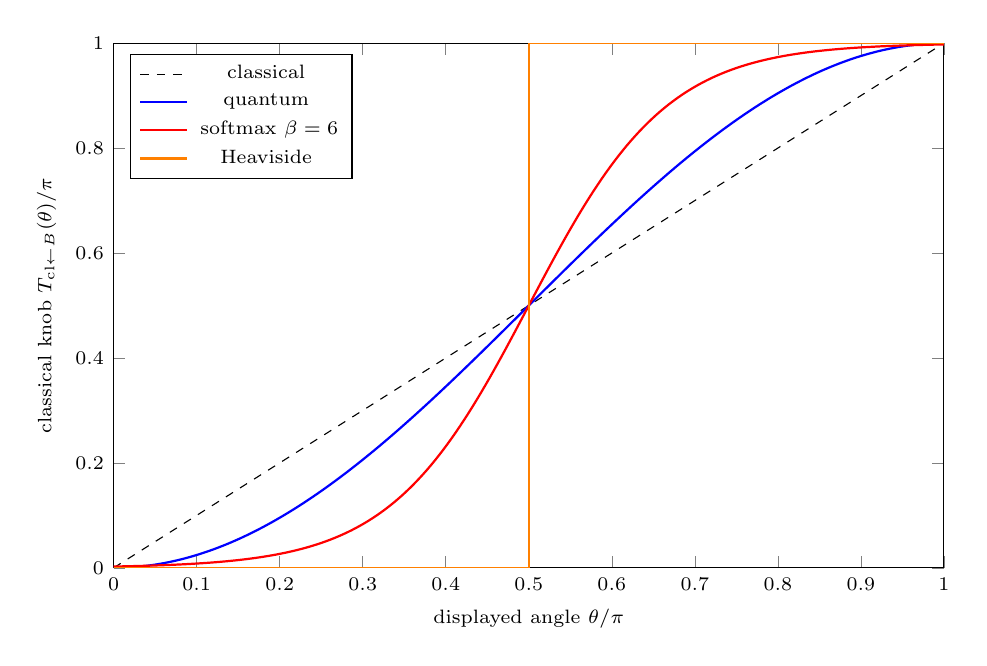
\begin{tikzpicture}
\begin{axis}[
    width=\columnwidth,
    height=0.68\columnwidth,
    xmin=0,xmax=1,
    ymin=0,ymax=1,
    xlabel={displayed angle \(\theta/\pi\)},
    ylabel={classical knob \(T_{{\rm cl}\leftarrow B}(\theta)/\pi\)},
    legend style={font=\scriptsize,at={(0.02,0.98)},anchor=north west},
    ticklabel style={font=\scriptsize},
    label style={font=\scriptsize},
    samples=200
]
\addplot[black,dashed,domain=0:1] {x};
\addlegendentry{classical}
\addplot[blue,thick,domain=0:1] {sin(90*x)^2};
\addlegendentry{quantum}
\addplot[red,thick,domain=0:1] {1/(1+exp(-6*(2*x-1)))};
\addlegendentry{$\;$softmax \(\beta=6\)}
\addplot[orange,thick] coordinates {(0,0) (0.5,0) (0.5,1) (1,1)};
\addlegendentry{Heaviside}
\end{axis}
\end{tikzpicture}
\end{center}
\caption{Classical inverse knobs for several target response laws.  Since
\(R_{\rm cl}(\tau)=\tau/\pi\), the transcribed classical knob is simply
\(T_{{\rm cl}\leftarrow B}(\theta)/\pi=R_B(\theta)\).  The curves show how a
linear classical response must be read on a generally non-symmetry-preserving
scale in order to mimic a quantum, softmax, or Heaviside response as a
function of the displayed angle.}
\label{fig:inverse-knobs}
\end{figure}

This single-curve trick should not be confused with a solution of a Bell or
Boole problem.  In a Bell--Clauser--Horne--Shimony--Holt (CHSH) experiment one does not merely fit one
function \(E(\theta)\).  One must assign probabilities to several settings at
once, such as \(a,b,a',b'\), with one common underlying distribution over
predetermined answers.  A separate inverse knob can make each pairwise
correlation look right, but those pairwise deformations need not come from one
global angle scale.  The failure is already visible in the cheat parameters:
\(T(\theta_1+\theta_2)\) generally differs from
\(T(\theta_1)+T(\theta_2)\).  Thus the deformed pairwise angles need not be
compatible with one geometry of four settings.  The marginal-extension problem
then reappears, and Farkas' lemma supplies the relevant obstruction.

The elastic-band examples make this warning concrete.  Aerts' spin machine and
its extended-Bloch descendants use a hidden break point, or more generally a
hidden measurement interaction, to generate Born-like responses from an
ordinary macroscopic mechanism~\cite{aerts-69,Aerts_2014,Aerts_2016}.  The
rubber-band analysis of context communication stresses the complementary
limitation: recovering a cosine-shaped pair correlation in one adapted
arrangement is not yet the same as a Bell-local simulation of a CHSH
family~\cite{svozil-2022-epr}.  If the band or share has to be realigned when
the selected pair \((a,b),(a,b'),(a',b),(a',b')\) changes, then the knob
transcription has become context communication.  The shadow can be made to
look quantum after breakfast, lunch, teatime, and supper, but the four shadows
no longer arise from one setting-independent joint valuation.  In Sven Aerts'
Popescu--Rohrlich (PR)-box rubber-band construction the same point appears in a more extreme form:
the resource is a single extended object whose breaking co-creates the two
outcomes~\cite{AertsSven}.  These models are therefore relevant here not as
refutations of Boole--Bell, but as physical parables of where the
response-function program stops: a single curve can be reparametrized, whereas
a Bell web requires one common nonadaptive geometry or else a genuinely
nonlocal or nonseparable resource.

\emph{Two contexts.---}
The same logic explains why two contexts, even when they share outcomes, are
not yet enough to force a probability-level obstruction.  Let
\begin{equation}
        A=S\cup X,\qquad B=S\cup Y
\end{equation}
be two Boolean blocks, with shared atoms \(S\), atoms \(X\) belonging only to
\(A\), and atoms \(Y\) belonging only to \(B\).  Suppose context-wise
probabilities \(p^A\) and \(p^B\) are normalized, nonnegative, and agree on
the overlap:
\begin{equation}
        p^A_s=p^B_s=:r_s\qquad (s\in S).
        \label{eq:overlap}
\end{equation}
Let \(m=1-\sum_{s\in S}r_s\).  Then
\begin{equation}
        \sum_{x\in X}p^A_x=m=\sum_{y\in Y}p^B_y .
\end{equation}
If \(m>0\), choose for example
\begin{equation}
        w_{xy}=\frac{p^A_x p^B_y}{m};
        \label{eq:two-context-coupling}
\end{equation}
if \(m=0\), set all \(w_{xy}=0\).  Now define a classical sample space with
one point \(\lambda_s\) of weight \(r_s\) for each shared atom \(s\), and one
point \(\lambda_{xy}\) of weight \(w_{xy}\) for each pair \(x\in X,y\in Y\).
At \(\lambda_s\), the shared atom \(s\) is the true answer in both contexts.
At \(\lambda_{xy}\), the answer to \(A\) is \(x\) and the answer to \(B\) is
\(y\).  Reading the \(A\)-coordinate gives \(p^A\), and reading the
\(B\)-coordinate gives \(p^B\).

\begin{proposition}
Every pair of normalized context distributions satisfying
Eq.~\eqref{eq:overlap} has a classical joint model over deterministic answers
for the two blocks.
\end{proposition}

This is just the elementary coupling theorem for two marginal distributions,
with the shared outcomes treated as already coupled.  Equivalently, after the
common mass has been fixed, each residual cell obeys the finite
Frechet--Hoeffding bounds
\begin{equation}
        \max(0,p^A_x+p^B_y-m)\le w_{xy}\le \min(p^A_x,p^B_y),
        \label{eq:frechet-hoeffding}
\end{equation}
and Eq.~\eqref{eq:two-context-coupling} is just one point in this coupling
polytope.  Thus two-context
intertwining has no nontrivial marginal obstruction at the level of static
weights.  The response functions realizing those weights may still be very
different: continuous or discontinuous, affine or Malus-type, softmax-shaped or
boundary-valued.  The obstruction requires a sufficiently constrained web of
local shadows, typically a cycle or a Kochen-Specker-type pasting, so that all
pairwise or context-wise agreements cannot be realized by one global
nonnegative distribution.

\emph{Farkas alternative.---}
The extension problem can be written in the form
\begin{equation}
        M q=b,\qquad q\ge 0 ,
        \label{eq:marginal-lp}
\end{equation}
where \(q\) is a distribution over deterministic global assignments and \(b\)
collects the observed context probabilities.  Farkas' lemma says that exactly
one of the following alternatives holds:
\begin{align}
&\exists q\ge 0 \text{ such that } Mq=b,                         \\
&\exists y \text{ such that } y^TM\ge 0 \text{ and } y^Tb<0 .
        \label{eq:farkas}
\end{align}
The second line is a separating inequality.  Garg and Mermin used precisely
this logic to formulate the question of whether specified pair distributions
can arise as marginals of compatible higher-order distributions
\cite{Garg1984}.  Fine's theorem for Bell inequalities is a celebrated special
case of the same joint-distribution viewpoint \cite{Fine-82}; Pitowsky's
correlation polytopes place the construction in convex-geometric form
\cite{pitowsky-86}.

Equation~\eqref{eq:marginal-lp} is also the finite-dimensional skeleton of
simplex embeddability tests.  A prepare-and-measure fragment is classical when
its probability table factors through a simplex, or equivalently through a
nonnegative cone generated by deterministic responses.  Vectorizing the
nonnegative factorization again yields a linear feasibility problem; infeasibility
has a Farkas dual certificate.  The recent generalized-probabilistic simplex
criteria and their linear-programming implementations make this operational
version explicit \cite{schmid-2021-simplex,selby-2024-lp}.

\emph{Simplex and theta bodies.---}
For a fixed exclusivity structure there are two natural convex bodies.  The
classical body is generated by deterministic two-valued states:
\begin{equation}
        \mathcal P_{\rm cl}=\conv\{\text{admissible }0/1\text{ assignments}\}.
\end{equation}
For graphs this is the stable-set polytope, denoted \(\STAB(G)\), possibly with
additional normalization equations for complete contexts.  One standard
realization of the corresponding quantum body is obtained from squared
projections of a state onto an orthogonal representation:
\begin{equation}
        p_v=|\langle\psi|v\rangle|^2 ,
\end{equation}
or by the corresponding density-operator formula.  In graph language this is
related to Lovasz-type theta bodies \cite{Lovasz1975,GroetschelLovaszSchrijver1986,cabello-severini-winter-2014}.
The larger admissible-weight body, often called the no-disturbance or
consistent-exclusivity polytope in contextuality language, is obtained by
keeping only nonnegativity, context-wise normalization, additivity on exclusive
events, and equality of values assigned to the same atom in different
contexts.

For one clique, these bodies have the same operational shadow: the simplex.
For two cliques pasted along a common clique, the explicit coupling above still
keeps the classical and quantum context marginals aligned.  Cycles change the
situation.  The pentagon is the minimal calibration.  Let
\[
        C_i=\{a_i,a_{i+1},x_i\},\qquad i=1,\ldots,5,
\]
with indices modulo \(5\).  The cyclic atoms \(a_i\) are the intertwining
observables, and the atoms \(x_i\) are context-specific.  The assignment
\begin{equation}
        p(a_i)=\frac12,\qquad p(x_i)=0
        \quad (i=1,\ldots,5)
        \label{eq:pentagon-half-weight}
\end{equation}
obeys completeness in every context,
\(p(a_i)+p(a_{i+1})+p(x_i)=1\), is additive on mutually exclusive events
inside each Boolean block, and is atom-consistent: the same intertwining atom
has the same value wherever it occurs.  This is deliberately weaker than
noncontextual hidden-variable embeddability in a classical simplex, and it is
not Spekkens-style operational noncontextuality.  Indeed, it is not a convex
mixture of deterministic two-valued states.

Indeed, the classical noncontextual bound on the five cyclic events is
\begin{equation}
        \sum_{i=1}^5 p_i\le 2,
\end{equation}
for the Klyachko--Can--Binicio\u{g}lu--Shumovsky (KCBS) pentagon inequality~\cite{Klyachko-2008,Badziag-2011,Bub-2009},
whereas a faithful quantum orthogonal representation reaches
\begin{equation}
        \sum_{i=1}^5 p_i=\sqrt{5}.
\end{equation}
This is the Lovasz number of the pentagon exclusivity graph
\cite{lovasz-79,cabello-severini-winter-2014}.
The half-weight~\eqref{eq:pentagon-half-weight} gives
\(\sum_i p(a_i)=5/2\), so it is admissible and atom-consistent, yet lies
beyond both the classical bound and the usual KCBS/Lovasz quantum value.
This is the KCBS/Lovasz-theta gap in its most economical form.  In the language used here,
the Hilbert-space squared-projection body has escaped the classical simplex
body only after enough context-wise shadows have been required to glue
together; the exotic half-weight escapes still farther inside the larger
admissible/no-disturbance polytope.  It is therefore best read as a boundary
object of the admissible theory, not as a Hilbert-space-realizable quantum
state.

For the pentagon this is also an explicit Farkas certificate.  Deterministic
classical assignments are the stable sets of \(C_5\), and each stable set
contains at most two cyclic atoms.  Hence the row vector
\(y=(1,1,1,1,1)\) separates the half-weight from the classical stable-set
polytope:
\begin{equation}
        y^T b=\frac52
        \quad\text{whereas}\quad
        \max_{\chi\in\STAB(C_5)} y^T\chi=2 .
        \label{eq:pentagon-farkas-certificate}
\end{equation}
Thus the KCBS inequality is precisely the Farkas dual witness for the
nonexistence of a nonnegative convex combination of deterministic valuations
realizing \(b=(1/2,\ldots,1/2)\).

The response-function point is sharpest in this example.  The half-weight may
be approached by a generalized softmax path
\begin{equation}
        p_r(a_i)=\frac{1}{2+r},\qquad
        p_r(x_i)=\frac{r}{2+r},
        \label{eq:pentagon-softmax-path}
\end{equation}
where \(r=g(t)/g(u_0)\).  The uniform state occurs at \(r=1\), and the exotic
half-weight is the boundary limit \(r\to0\).  For an exponential softmax this
is a limiting response rather than a finite-score response; for a Heaviside
link one instead obtains a discontinuous knob response.  The admissibility
equations are the same in all cases, but the response function---the behavior
of the knob---is very different.

\emph{Informal summary.---}
The moral is not that quantum probability is secretly classical, nor that a
single probability vector contains enough information to reveal its origin.
The moral is more local: one must keep track of what has been thrown away.
When the generating geometry is forgotten, a single context leaves only a
shadow.  When the physical knob is retained, the shadow begins to move, and
its calibrated, symmetry-constrained motion can already distinguish affine
classical response from Malus-type Hilbert-space response or from
discontinuous threshold behavior.

Two weakly pasted shadows still need not betray anything nonclassical.  If two
contexts agree on their shared atoms, the remaining mass can be coupled by an
ordinary joint distribution.  The obstruction appears only when enough local
shadows are required to hang together as one global object.  Then the question
becomes a linear feasibility problem: either there is a classical joint model
or simplex factorization, or Farkas' lemma supplies the separating inequality.
The rubber-band models are the laboratory parable: with context communication,
adaptive realignment, or one extended nonseparable band, they can produce
quantum-looking shadows, but not a single Bell-local valuation glued across
all four settings.

Thus the staged picture is: shadow, calibrated knob, weak pasting, global web.
The frozen shadow hides classical, quantum, and exotic origins.  The knob
records how the shadow changes under symmetry-constrained variation.  Weak
pastings remain extendable.  Rich webs can fail to extend.  The pentagon
half-weight finally reminds us that admissibility and atom-consistency are
still not the same as classical embeddability or as a physical response law:
the same static constraints can be obeyed by very different knobs.

\begin{acknowledgments}
This research was funded in whole or in part by the \textit{Austrian Science Fund (FWF)} [Grant \href{https://doi.org/10.55776/PIN5424624}{digital object identifier (DOI): 10.55776/PIN5424624}].
The author acknowledges TU Wien Bibliothek for financial support through its Open Access Funding Programme.

This text was partially created and revised with assistance from large language models. All content, ideas, and prompts were provided by the author.
\end{acknowledgments}

\bibliography{svozil}

\end{document}
